\documentclass{article}
\usepackage[a4paper]{geometry}
\usepackage{amsmath}
\usepackage{amsfonts}
\usepackage{amssymb}
\usepackage{graphicx}
\usepackage{subcaption}
\usepackage{float}
\graphicspath{{./images/}}
\begin{document}
\begin{center}
	{\LARGE Exercise 5}\linebreak
	{\large [Avik Banerjee (3374885), Soumyadeep Bhattacharjee (3375428)]}
\end{center}
\textit{Text in italics are notes taken during the exercise}
\section{Random Walk}
The value of each state is initialized to 0.5 before the first episode starts, while the final states are set to 0.
In the first epoch, as we proceed from $C \rightarrow A$, $V(S_t)$ results in 0 for states C and B, as both the previous and current states have $V(S) = 0.5$.
However, when transitioning from A to the leftmost state, the value functions for the consecutive states are not the same.
	\begin{equation*}
	\begin{split}
	&V(S_t) \leftarrow V(S_t) + \alpha [R_{t+1} + \gamma V(S_{t+1}) - V(S_t)]\\
	&\text{where}\; V(S_t) = 0.5, V(S_{t+1}) = 0 
	\end{split}
	\end{equation*}			
Plugging in all the remaining values, we get $V(S_t) = 0.45$, whereby the value changes by 0.05.
\section{Sarsa and Q-learning on the FrozenLake}
\begin{enumerate}
	\item[a)] The state-value function, action-value function for Sarsa are as follows:
	\begin{figure}[H]
	\begin{subfigure}[b]{0.5\linewidth}
		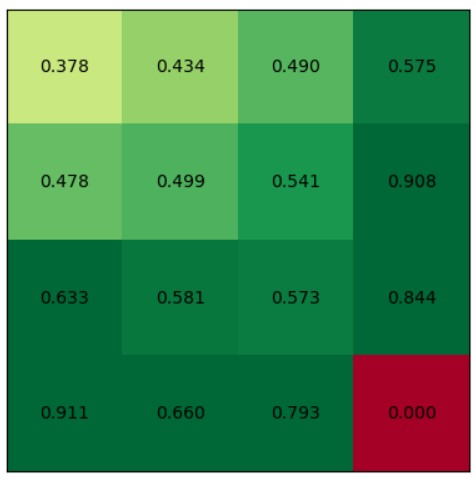
\includegraphics[width = \linewidth]{SarsaV1.jpg}
		\caption{State-value function}
	\end{subfigure}
	\begin{subfigure}[b]{0.5\linewidth}
		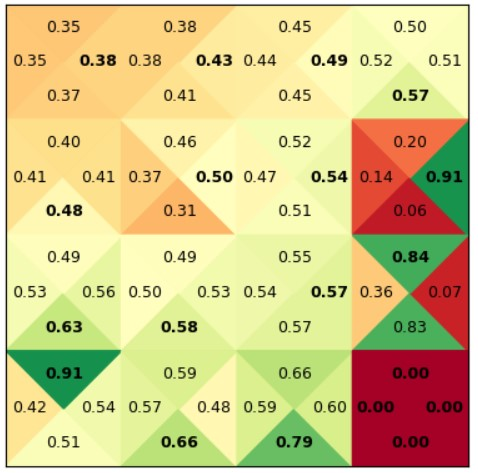
\includegraphics[width = \linewidth]{SarsaQ1.jpg}
		\caption{Action-value function}
	\end{subfigure}
	\end{figure}
The policy:
\begin{figure}[H]
	\centering
	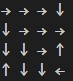
\includegraphics{SarsaPolicy1.jpg}
\end{figure}
The average episode length over every 100 episodes:
\begin{figure}[H]
	\centering
	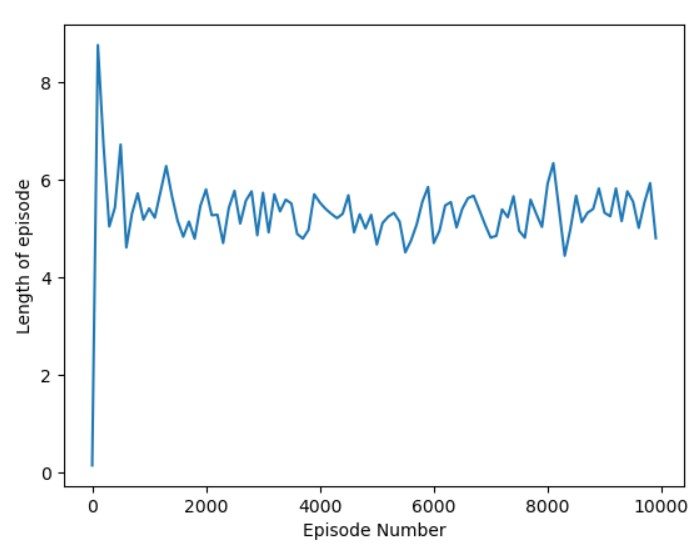
\includegraphics[scale = 0.5]{SarsaPlot1.jpg}
\end{figure}
\item[b)] The state-value function, action-value function for Q-learning are as follows:
\begin{figure}[H]
	\begin{subfigure}[b]{0.5\linewidth}
		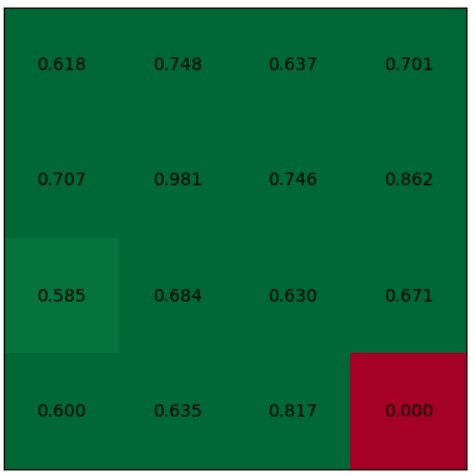
\includegraphics[width = \linewidth]{QV1.jpg}
		\caption{State-value function}
	\end{subfigure}
	\begin{subfigure}[b]{0.5\linewidth}
		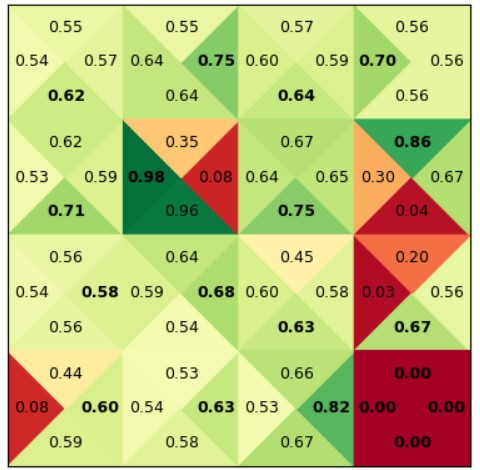
\includegraphics[width = \linewidth]{QQ1.jpg}
		\caption{Action-value function}
	\end{subfigure}
\end{figure}
The policy:
\begin{figure}[H]
	\centering
	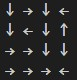
\includegraphics{QPolicy1.jpg}
\end{figure}
The average episode length over every 100 episodes:
\begin{figure}[H]
	\centering
	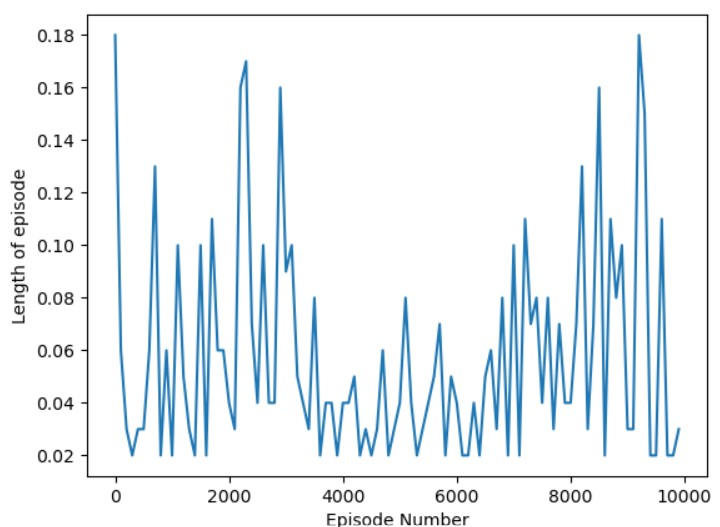
\includegraphics[scale = 0.5]{QPlot1.jpg}
\end{figure}
As is evident from the episode-length graphs, the optimal policy obtained at the end of 10000 iterations may not have the lowest episode length, there are multiple minima that are reached before all episodes are covered.
\textit{Sarsa actually converges to an optimal version of the epsilon-greedy policy since it is on-policy, whereas Q-learning, being on-policy converges to the actual optimal policy.}
\item[c)] The non-slippery version makes the episode lengths converge faster, which means the optimal policy is derived faster, which is prominently visible in the episode-length plot of Q-learning.\linebreak
The state-value function, action-value function for Sarsa are as follows:
\begin{figure}[H]
	\begin{subfigure}[b]{0.5\linewidth}
		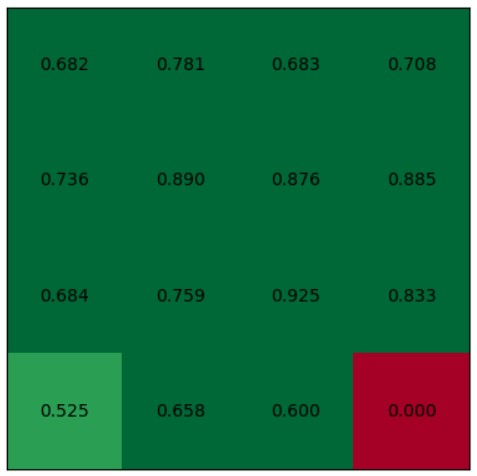
\includegraphics[width = \linewidth]{SarsaV2.jpg}
		\caption{State-value function}
	\end{subfigure}
	\begin{subfigure}[b]{0.5\linewidth}
		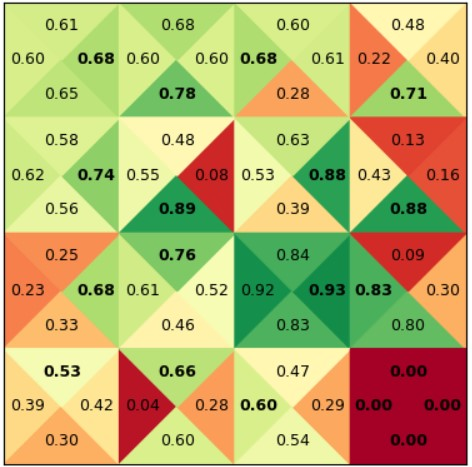
\includegraphics[width = \linewidth]{SarsaQ2.jpg}
		\caption{Action-value function}
	\end{subfigure}
\end{figure}
The policy for Sarsa:
\begin{figure}[H]
	\centering
	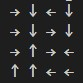
\includegraphics{SarsaPolicy2.jpg}
\end{figure}
The average episode length over every 100 episodes:
\begin{figure}[H]
	\centering
	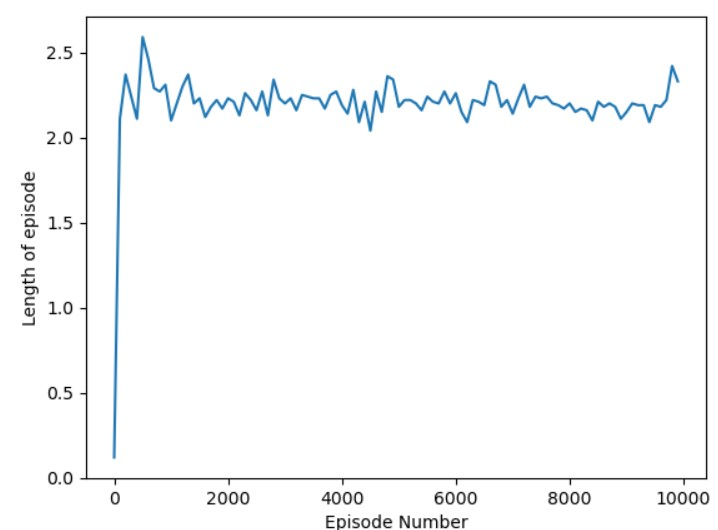
\includegraphics[scale = 0.5]{SarsaPlot2.jpg}
\end{figure}
The state-value function, action-value function for Q-learning are as follows:
\begin{figure}[H]
	\begin{subfigure}[b]{0.5\linewidth}
		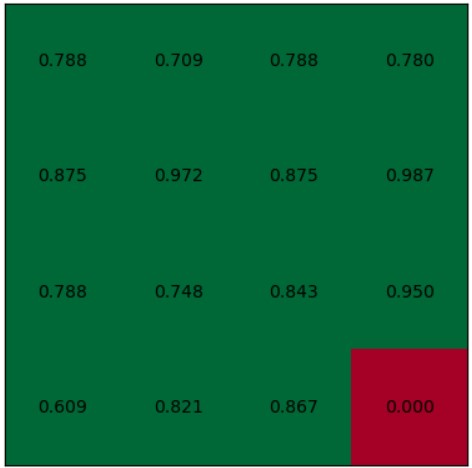
\includegraphics[width = \linewidth]{QV2.jpg}
		\caption{State-value function}
	\end{subfigure}
	\begin{subfigure}[b]{0.5\linewidth}
		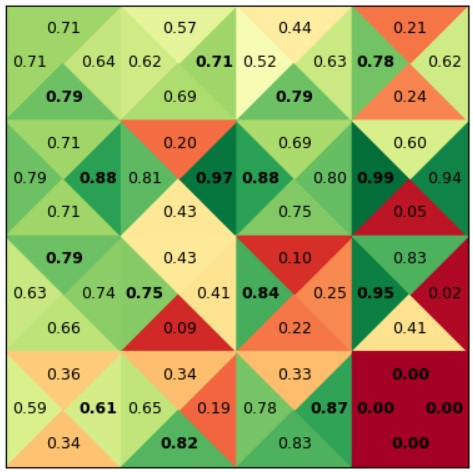
\includegraphics[width = \linewidth]{QQ2.jpg}
		\caption{Action-value function}
	\end{subfigure}
\end{figure}
The policy:
\begin{figure}[H]
	\centering
	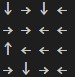
\includegraphics{QPolicy2.jpg}
\end{figure}
The average episode length over every 100 episodes:
\begin{figure}[H]
	\centering
	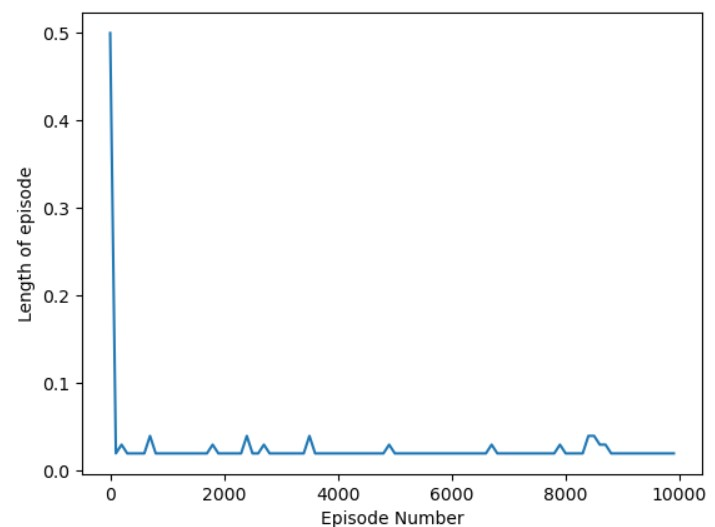
\includegraphics[scale = 0.5]{QPlot2.jpg}
\end{figure}
\item[d)]The state-value function, action-value function for Sarsa are as follows:
\begin{figure}[H]
	\begin{subfigure}[b]{0.5\linewidth}
		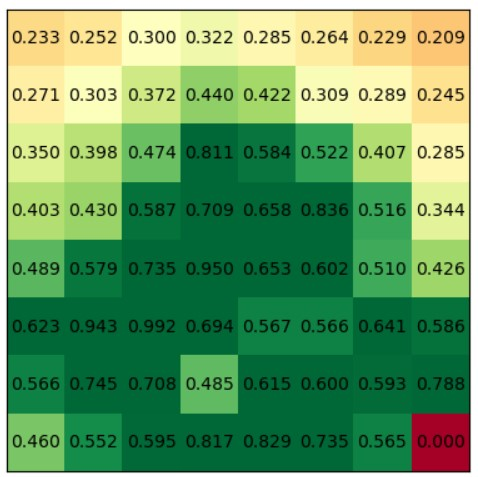
\includegraphics[width = \linewidth]{SarsaV3.jpg}
		\caption{State-value function}
	\end{subfigure}
	\begin{subfigure}[b]{0.5\linewidth}
		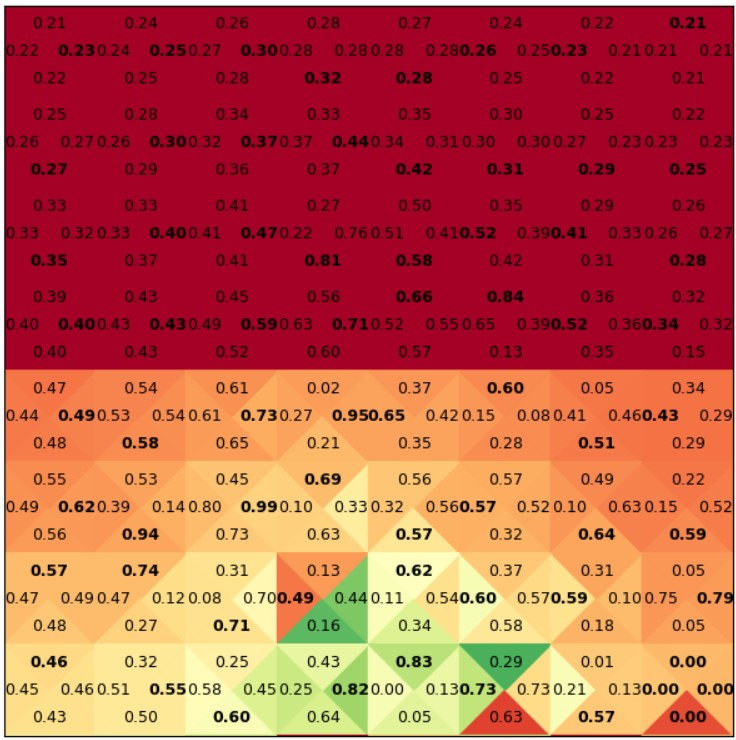
\includegraphics[width = \linewidth]{SarsaQ3.jpg}
		\caption{Action-value function}
	\end{subfigure}
\end{figure}
The policy for Sarsa:
\begin{figure}[H]
	\centering
	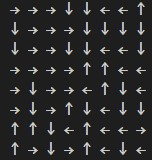
\includegraphics{SarsaPolicy3.jpg}
\end{figure}
The average episode length over every 100 episodes:
\begin{figure}[H]
	\centering
	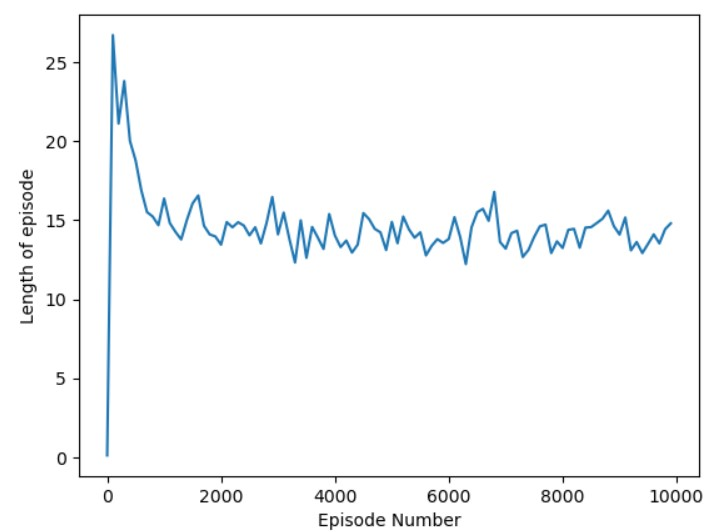
\includegraphics[scale = 0.5]{SarsaPlot3.jpg}
\end{figure}
The state-value function, action-value function for Q-learning are as follows:
\begin{figure}[H]
	\begin{subfigure}[b]{0.5\linewidth}
		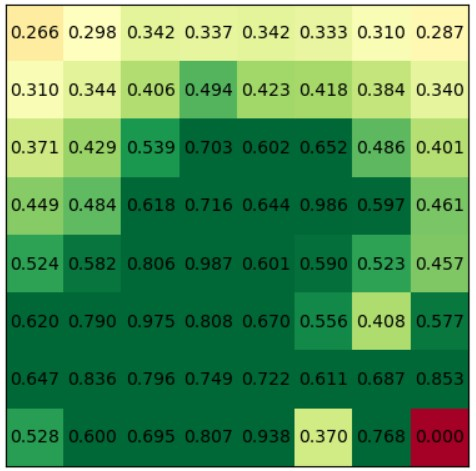
\includegraphics[width = \linewidth]{QV3.jpg}
		\caption{State-value function}
	\end{subfigure}
	\begin{subfigure}[b]{0.5\linewidth}
		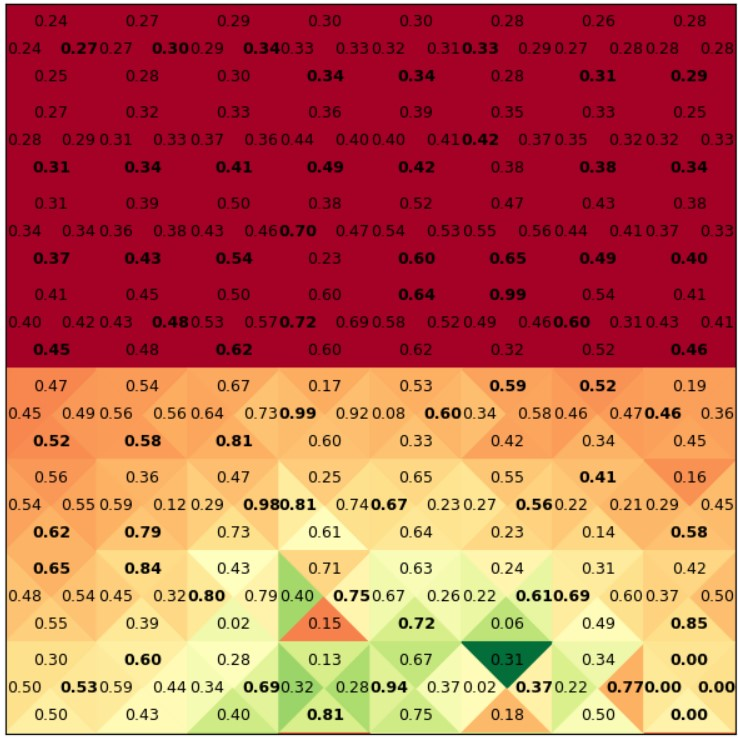
\includegraphics[width = \linewidth]{QQ3.jpg}
		\caption{Action-value function}
	\end{subfigure}
\end{figure}
The policy:
\begin{figure}[H]
	\centering
	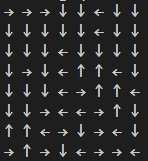
\includegraphics{QPolicy3.jpg}
\end{figure}
The average episode length over every 100 episodes:
\begin{figure}[H]
	\centering
	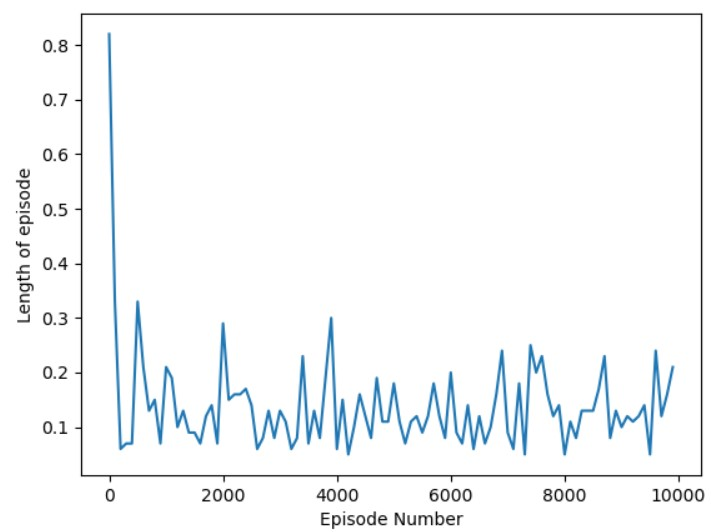
\includegraphics[scale = 0.5]{QPlot3.jpg}
\end{figure}
\end{enumerate}
\end{document}